% !TEX root = ../../main.tex


\begin{figure}[!htb]
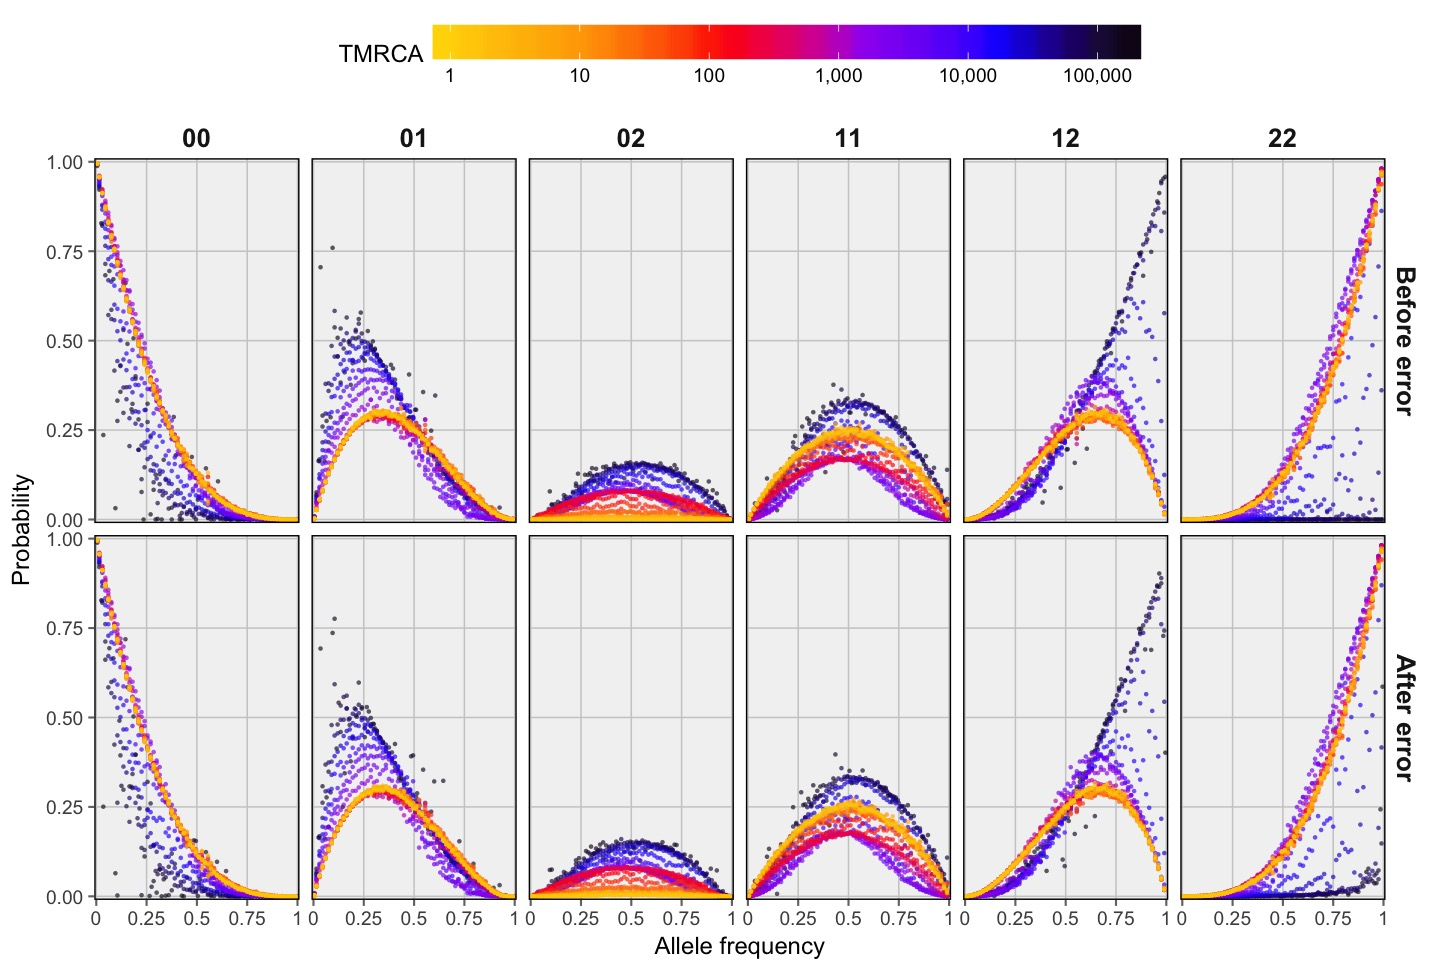
\includegraphics[width=\textwidth]{./img/ch4/emission_tmrca_reduced_new}
\Caption{Empirical emission probabilities of genotype pairs dependent on time}
{The relative proportions of genotype pairs observed in IBD segments in simulated data are shown, which is distinguished by the \glsentryfull{tmrca}; \ie the time since a haplotype was co-inherited from a common ancestor.
The dataset used to determine proportions was the original, error-free dataset ($D$).
Dots indicate the empirical mean proportion by allele frequency bin (${n=100}$), equally spaced along the frequency spectrum.
Genotype pairs are colour-coded (see legend).
Shaded areas indicate the space between the expected frequency distribution under IBD and non-IBD, coloured according to the respective genotype pair, where the edges of these areas correspond to the expectation under IBD (\emph{dashed}) and non-IBD (\emph{dotted}).\CorrectLabel}
{fig:emission_tmrca}
\end{figure}
